\documentclass[11pt,letterpaper]{article}
\usepackage[lmargin=1in,rmargin=1in,bmargin=1in,tmargin=1in]{geometry}
\usepackage{style/quiz}
\usepackage{style/commands}

% -------------------
% Content
% -------------------
\begin{document}
\thispagestyle{title}


% Quiz 1
\quizsol \textit{True/False}: Both $12= 3 \cdot 4$ and $12= 2^2 \cdot 3$ are prime factorizations of 12.  \pspace

\sol The statement is \textit{false}. A factorization of an integer $n$ is a product of integers that yields $n$. For instance, if $n= 100$, then $n= 1 \cdot 100, 10 \cdot 10, 5 \cdot 20, \ldots$ are all factorizations of 100. A prime factorization is a factorization where all the numbers in the product are primes or powers of primes. [If $n$ is prime, we allow $n= n$ to be the prime factorization, i.e. the `empty' product.] Then in the instance of $n= 100$, the factorizations $5 \cdot 20$ cannot be a prime factorization because 20 is not prime. In the given problem, $12= 3 \cdot 4$ is \textit{not} a prime factorization because 4 is not prime ($4= 2 \cdot 2$), while $12= 2^2 \cdot 3$ is a prime factorization because we have written 12 as a product of (powers of) primes. By the Fundamental Theorem of Arithmetic, every integer greater than 1 is either prime or can be written uniquely (up to order, e.g. $6= 2 \cdot 3= 3 \cdot 2$) as a product of primes. \pvspace{1.5cm}



% Quiz 2
\quizsol \textit{True/False}: $\gcd(2^{50} \cdot 3^{60} \cdot 7^{40}, 2^{30} \cdot 3^{70} \cdot 5^{90})= 2^{30} \cdot 3^{60} \cdot 5^{90} \cdot 7^{40}$ \pspace

\sol The statement is \textit{false}. If one wishes to compute $\gcd(a, b)$, one can compute the prime factorizations of $a, b$ and find the product of the primes appearing in \textit{both} prime factorizations of $a, b$, each to the smaller of the prime powers involved in the factorizations of $a, b$. For instance, if we wanted to compute $\gcd(2520, 74844)= \gcd(2^3 \cdot 3^2 \cdot 5^1 \cdot 7, 2^2 \cdot 3^5 \cdot 7 \cdot 11)$, observe that the primes occurring both are $2, 3, 7$. The smallest power for each is 2, 2, 1, respectively. Therefore, $\gcd(2520, 74844)= \gcd(2^3 \cdot 3^2 \cdot 5^1 \cdot 7, 2^2 \cdot 3^5 \cdot 7 \cdot 11)= 2^2 \cdot 3^2 \cdot 7^1= 252$. In the given problem, while the smallest power of each prime was chosen, \textit{every} prime was used rather than just the primes both factorizations have in common. \pvspace{1.5cm}



% Quiz 3
\quizsol \textit{True/False}: We compute the reduced result of $(3/7)/(45/56)$ as follows: 
	\[
	\dfrac{\;\;\dfrac{3}{7}\;\;}{\dfrac{45}{56}}= \dfrac{3}{7} \cdot \dfrac{56}{45}= \dfrac{3 \cdot 56}{7 \cdot 45}= \dfrac{168}{315}
	\] \pspace

\sol The statement is \textit{false}. While the given answer is equal to the reduced answer, the given answer is not reduced (for instance, the numerator and denominator are both divisible by 3). Therefore, the statement is false. Remember, one should always cancel wherever possible \textit{before} `multiplying straight across' in multiplication of rational numbers:
	\[
	\dfrac{\;\;\dfrac{3}{7}\;\;}{\dfrac{45}{56}}= \dfrac{3}{7} \cdot \dfrac{56}{45}= \dfrac{\cancel{3}^1}{\cancel{7}^1} \cdot \dfrac{\cancel{56}^{\,8}}{\cancel{45}^{\,15}}= \dfrac{1}{1} \cdot \dfrac{8}{15}= \dfrac{1 \cdot 8}{1 \cdot 15}= \dfrac{8}{15}
	\] 





\newpage





% Quiz 4
\quizsol \textit{True/False}: 
	\[
	\dfrac{x y^4 z^3}{z^{-3} \sqrt{x^2 y^4}}= \dfrac{1}{\sqrt{x}}
	\] \pspace

\sol The statement is \textit{false}. We can simplify this expression as follows:
	\[
	\dfrac{x y^4 z^3}{z^{-3} \sqrt{x^2 y^4}}= \dfrac{x y^4 z^3}{z^{-3} (x^{2/2} y^{4/2})}= \dfrac{x y^4 z^3}{z^{-3} x y^2}= \dfrac{x y^4 z^3 z^3}{x y^2}= \dfrac{y^4 z^6}{y^2}= y^2 z^6
	\] \pvspace{1.2cm}



% Quiz 5
\quizsol \textit{True/False}: To compute 560 increased by 160\%, one computes $560(2.60)= 1456$. \pspace

\sol The statement is \textit{true}. To compute a percentage increase/decrease of a number $N$, we compute $N(1 \pm \%_d)$, where $N$ is the number, $\%_d$ is the percentage written as a decimal, and where we choose `$+$' if it is a percentage increase and `$-$' if it is a percentage decrease. So here, we compute\dots
	\[
	N(1 \pm \%_d)= 560(1 + 1.60)= 560(2.60)= 1456
	\] \pvspace{1.2cm}



% Quiz 6
\quizsol \textit{True/False}: Suppose a course has three exams: two prelims and a final exam. The final exam is worth twice as much as any of the other exams. If a student receives an 85\%, 89\%, and 81\% on the prelims and final exam, respectively, then their exam average is $85\% \left( \frac{1}{4} \right) + 89\%  \left( \frac{1}{4} \right) +  81\% \left( \frac{1}{2} \right)= 84\%$. \pspace

\sol The statement is \textit{true}. We know that the weighted average is $\sum \text{value} \cdot \text{weight}$. If the first exam is worth 1 part of the exam grade, the second must be worth 1 part and the final exam must be worth 2 parts (because it needs to be worth twice as much as either of the other two). Then the exam grade is split into $1 + 1 + 2= 4$ parts, which the first exam worth $1/4$~th of the grade, the second worth $1/4$~th of the grade, and the last worth $2/4= 1/2$ the grade. But then we have\dots
	\[
	\sum \text{value} \cdot \text{weight}= 85\% \cdot \frac{1}{4} + 89\% \cdot \frac{1}{4} + 81\% \cdot \frac{1}{2}= 21.25\% + 22.25\% + 40.5\%= 84\%
	\] \pvspace{1.2cm}



% Quiz 7
\quizsol \textit{True/False}: The acceleration towards Earth due to gravitational attraction is approximately 9.8~m/s$^2$. To convert this to feet per hour, you need to multiply 9.8~m/s$^2$ by $60^2/0.3048 \approx 11811.0236$. [1~ft = 0.3048~m] \pspace

\sol The statement is \textit{false}. To perform the conversion, we have\dots \par
	\begin{table}[!ht]
	\centering
	\hspace{-1cm}
	\begin{tabular}{c|c|c|c|c|c}
	9.8~m	& 1~ft		& 60~s   & 60~min & 60~s    & 60~min \\ \hline
	1~s$^2$	& 0.3048~m	& 1~min & 1~hr      & 1~min &  1~hr
	\end{tabular}
	\end{table} \par
which gives us\dots
	\[
	9.8 \cdot 60 \cdot 60 \cdot 60 \cdot 60/0.3048= 9.8 \cdot 60^4/0.3048 \text{ ft}/\text{hr}^2 \approx 16692913.38 \text{ ft}/\text{hr}^2
	\]
So we need multiply by $60^4/0.3048$, not $60^2/0.3048$. The given computation only converts one units of seconds to hours, leaving one unit of seconds unconverted. Therefore, the given answer is really 9.8~m/s$^2$ $\cdot$ $60^2/0.3048 \approx 11811.0236$~ft/(s $\cdot$ hr). \pvspace{1.4cm}



% Quiz 8
\quizsol \textit{True/False}: A function is a relation which has one output per input. \pspace

\sol The statement is \textit{true}. The definition of a function is as follows: a relation $f(x)$ is a function if for each input $x$, there is only one possible output, $f(x)$. For instance, the relation $f(x)$ shown below is a function because for each possible input, namely $2$, $4$, $6$, there is only one output, namely $f(2)= 8$, $f(4)= 4$, and $f(6)= 4$, respectively. 
	\[
	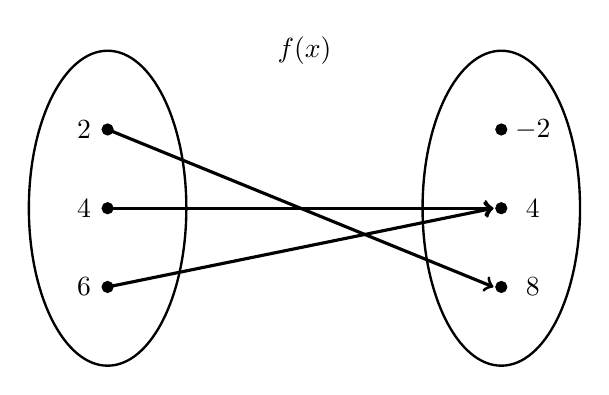
\begin{tikzpicture}
	\node at (2.5,2) {$f(x)$};
	% Ellipses
	\draw[line width=0.03cm] (0,0) circle (1 and 2);
	\draw[line width=0.03cm] (5,0) circle (1 and 2);
	
	% Nodes
	\draw[fill=black] (0,1) circle (0.07);
	\draw[fill=black] (0,0) circle (0.07);
	\draw[fill=black] (0,-1) circle (0.07);
	
	\draw[fill=black] (5,1) circle (0.07);
	\draw[fill=black] (5,0) circle (0.07);
	\draw[fill=black] (5,-1) circle (0.07);
	
	% Arrow
	\draw[line width=0.04cm,->] (0,1) -- (4.9,-1);
	\draw[line width=0.04cm,->] (0,0) -- (4.9,0);
	\draw[line width=0.04cm,->] (0,-1) -- (4.9,0);
	
	% Labels
	\node at (-0.3,1) {$2$};
	\node at (-0.3,0) {$4$};
	\node at (-0.3,-1) {$6$};
	
	\node at (5.4,1) {$-2$};
	\node at (5.4,0) {$4$};
	\node at (5.4,-1) {$8$};
	\end{tikzpicture}
	\]
As another example, $g(x)= \dfrac{x^2 + 4}{x^2 + x + 20}$ is a function because for each possible input, $x$, there is only one possible output---namely, the one obtained by `plugging in' $x$ and following order of operations in $g(x)$. \pvspace{1.4cm}



% Quiz 9
\quizsol \textit{True/False}: If $f(x)$ and $g(x)$ are functions, then $(f \circ g)(0)= (g \circ f)(0)$. \pspace

\sol The statement is \textit{false}. Function composition is not like multiplication---it is not commutative. So while $(fg)(0)= (gf)(0)$, it is not necessarily true that $(f \circ g)(0)= (g \circ f)(0)$. For instance, if $f(x)= 1$ and $g(x)= 2$, we have $(f \circ g)(0)= f(g(0))= f(2)= 1$ while $(g \circ f)(0)= g(f(0))= g(1)= 2$. While there can be particular choices of functions $f(x)$ and $g(x)$ such that $(f \circ g)(0)= (g \circ f)(0)$, it is not generally true, i.e. it is not true for all functions $f(x)$ and $g(x)$. \pvspace{1.4cm}



% Quiz 10
\quizsol \textit{True/False}: Suppose $f(x)$ is a function with $f(-2)= 10$ and $f(5)= 10$. This data is enough to show that $f^{-1}(x)$ does not exist. \pspace

\sol The statement is \textit{false}. If $f(-2)= 10$, then we know that $f^{-1}(10)= -2$. However, we also know that $f(5)= 10$ implies that $f^{-1}(10)= 5$. But we cannot have $f^{-1}(10)= -2$ and $f^{-1}(10)= 5$ at the same time---$f^{-1}(10)$ can only have one possible output if $f^{-1}(x)$ is a function. Because $f^{-1}(10)$ is not well defined, we know that $f^{-1}(x)$ is not a function, i.e. $f^{-1}(x)$ does not exist. 





\newpage




% Quiz 11
\quizsol \textit{True/False}: Any linear function can be written in the form $f(x)= mx + b$ for some $m, b$. \pspace

\sol \sol The statement is \textit{true}. A linear function has a constant rate of change. Suppose the rate of change were 5 and the current value is 2. After one step in time, the value is $2 + 1(5)= 2 + 5= 7$. After another step in time, the value is $7 + 5= 12$, or $2 + 2(5)= 2 + 10= 12$. Generally, after $n$ steps, the value is $2 + n \cdot 5= 5n + 2$, which is a linear function of the form $f(x)= mx + b$ with $x= n$ and $b= 2$. Generally, if we start with initial value $y_0$ and have a constant rate of change $m$, after $x$ steps, we have $y= y_0 + x \cdot m= mx + y_0$. This is a linear function with $y= y$, $x= x$, $m= m$, and $b= y_0$. But then we see that `any' function which changes at a constant rate is a linear function. We know that a linear function $f(x)= mx + b$ has a constant rate of change---the slope $m$. Therefore, a function is linear if and only if it has a constant rate of change. \pvspace{1.5cm}



% Quiz 12
\quizsol \textit{True/False}: The equation of a line through a point $(x_0, y_0)$ with slope $m$ is given by $y= y_0 + m(x - x_0)$, where $y_0$ represents some initial value and $m(x - x_0)$ represents a net change in $y_0$. \pspace

\sol The statement is \textit{true}. Observe that the function is linear: $y= y_0 + m(x - x_0)= y_0 + mx - mx_0= mx + (y_0 - mx_0)$ with $m= m$ and $b= y_0 - mx_0$. Observe that when $x= x_0$, we have $y= y_0 + m(x_0 - x_0)= y_0 + m(0)= y_0$ so that the line contains the point $(x_0 , y_0)$. Therefore, $y= y_0 + m(x - x_0)$ is a line with slope $m$ passing through the point $(x_0, y_0)$. Now $m$ is the amount that $y$ changes if $x$ changes. The amount of change in $x$ is $x - x_0$. Therefore, $m(x - x_0)$ is the net change in the initial value $y_0$. 














\end{document}